\documentclass[12pt,a4paper]{article}

% --------------------------------------------------
% PAQUETES
% --------------------------------------------------
\usepackage[utf8]{inputenc}
\usepackage[T1]{fontenc}
\usepackage[spanish]{babel}
\usepackage{graphicx}
\usepackage{geometry}
\usepackage{hyperref}
\usepackage{url}
\usepackage{array}
\usepackage{float}

\geometry{
    top=1.5cm,
    bottom=1.5cm,
    left=2cm,
    right=2cm
}

\hypersetup{
    colorlinks=true,
    urlcolor=blue,
    linkcolor=black
}

\pagestyle{empty}

\begin{document}

% ==================================================
% CARÁTULA
% ==================================================

\begin{center}

{\Large \textbf{UNIVERSIDAD TÉCNICA ESTATAL DE QUEVEDO}}\\[0.2cm]

{\large Facultad de Ciencias de la Ingeniería}\\
{\large Carrera de Ingeniería de Software}\\[0.5cm]

\rule{\textwidth}{0.6pt}\\[0.4cm]

{\LARGE \textbf{PRUEBA PRÁCTICA --- UNIDAD IV}}\\[0.2cm]

{\large Validación, Gestión, Herramientas y Estándares de Requisitos}\\[0.5cm]

\rule{\textwidth}{0.6pt}\\[0.5cm]

\begin{tabular}{>{\bfseries}p{4.2cm} p{10cm}}
Asignatura: & Ingeniería de Requisitos (ISR-401) \\[0.15cm]
Estudiante: & Vaca Romero David Octavio \\[0.15cm]
Curso: & 4to Nivel --- Paralelo A \\[0.15cm]
Fecha: & 11 de agosto de 2026 \\[0.15cm]
Docente: & Ing. Gleiston Guerrero, Mg. \\[0.15cm]
Caso práctico: & Sistema de Gestión de Pedidos \\
\end{tabular}

\vspace{0.45cm}

{\bfseries Repositorio GitHub:}\\[0.15cm]

\resizebox{0.97\textwidth}{!}{
\href{https://github.com/David-Bs1/Evaluacion-IR-Unidad-IV-VacaDavid}
{\texttt{https://github.com/David-Bs1/Evaluacion-IR-Unidad-IV-VacaDavid}}
}

\vspace{0.45cm}

{\large \textbf{Captura del resumen del cuestionario SGA}}\\[0.15cm]

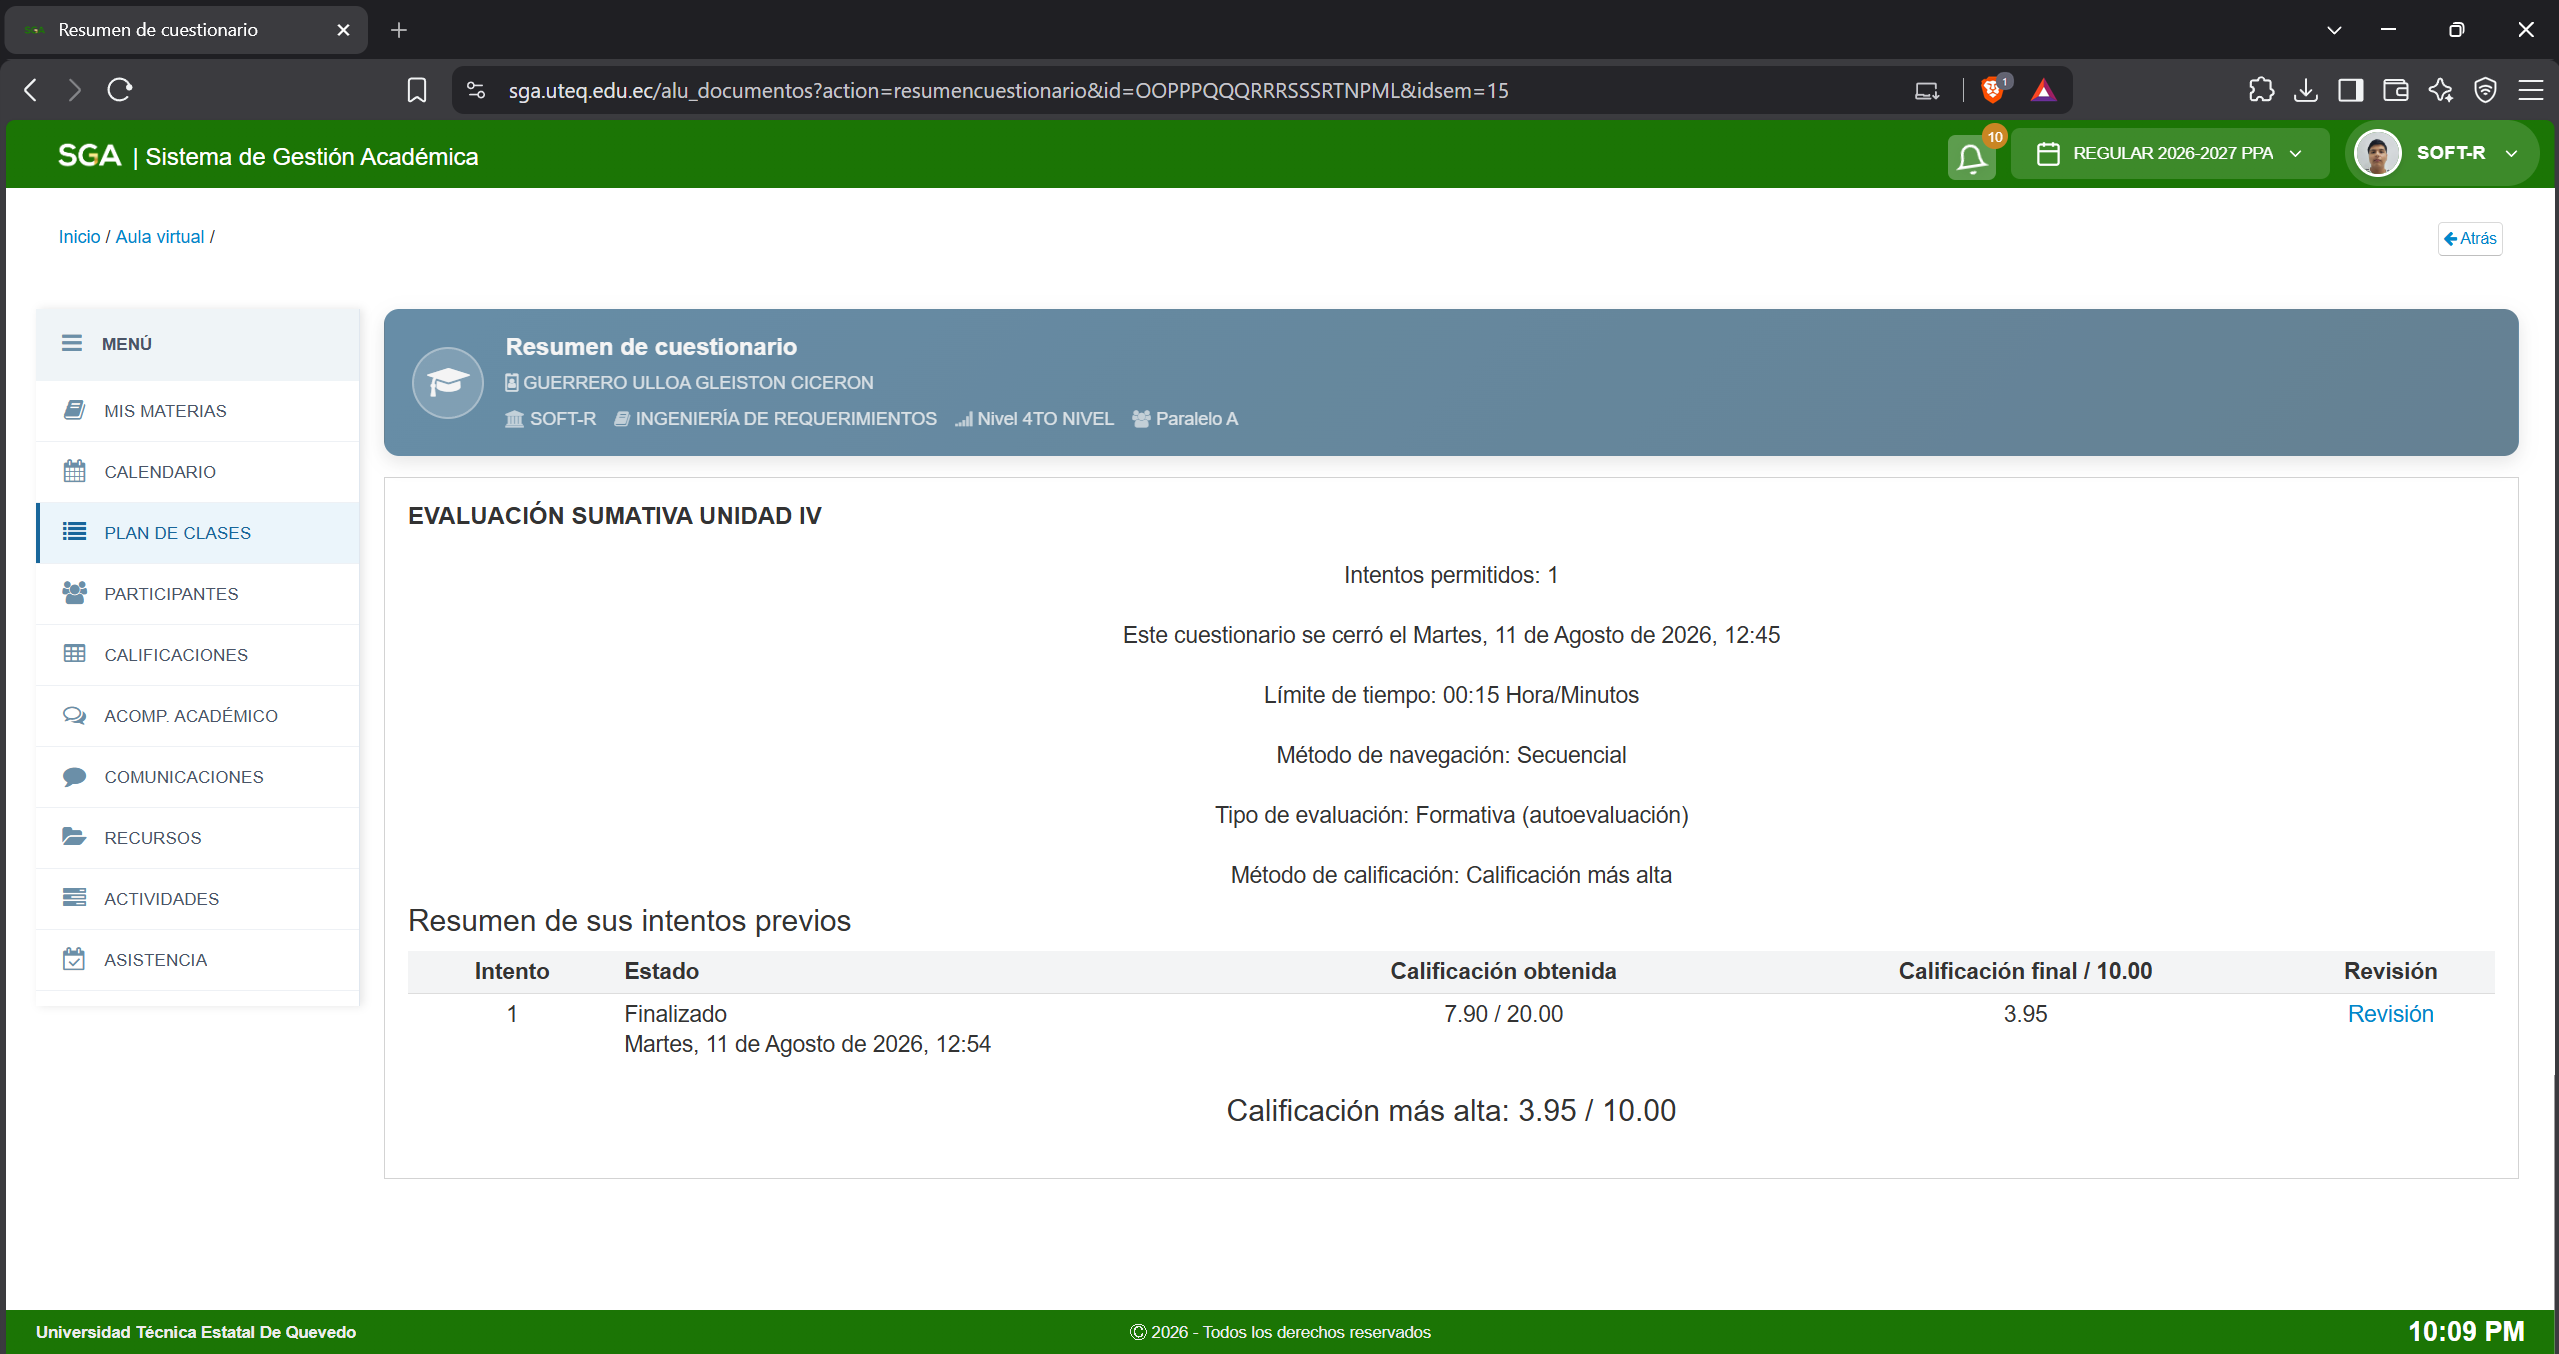
\includegraphics[
    width=0.90\textwidth,
    height=5.0cm,
    keepaspectratio
]{figuras/resumen_cuestionario_sga.png}

\vspace{0.25cm}

{\large \textbf{Captura de la evaluación del intento SGA}}\\[0.15cm]

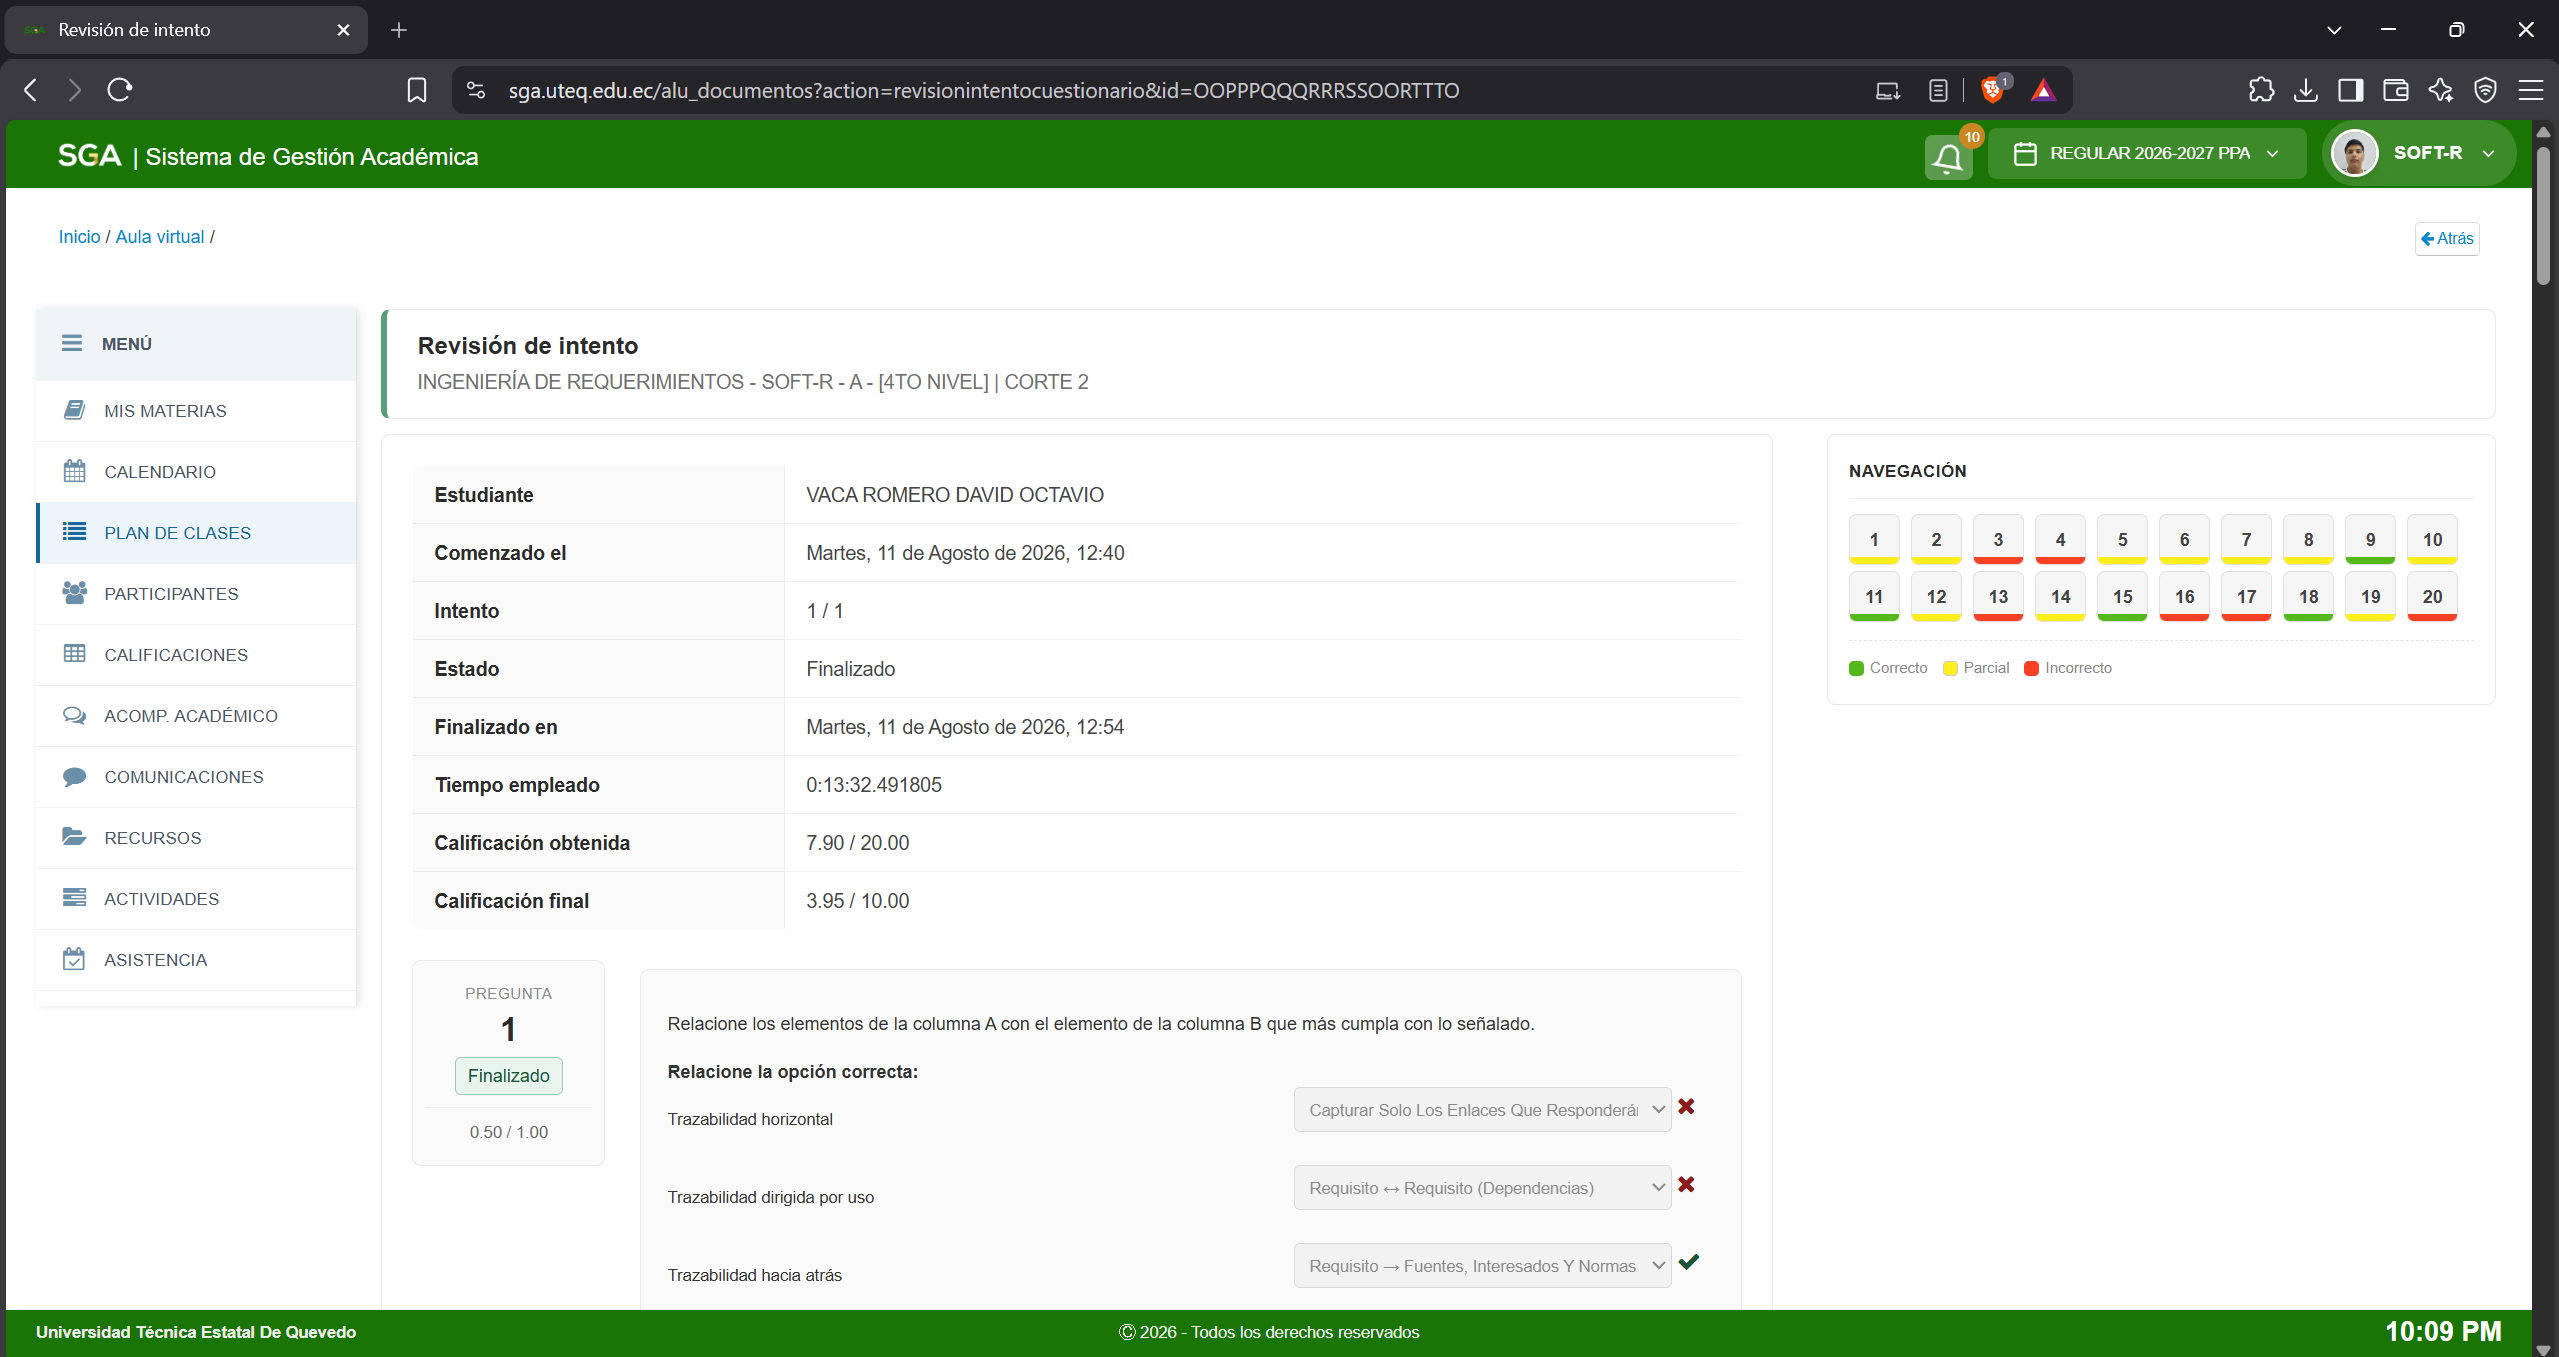
\includegraphics[
    width=0.90\textwidth,
    height=5.0cm,
    keepaspectratio
]{figuras/revision_intento_sga.png}

\end{center}

% ==================================================
% AQUÍ COMENZARÁ POSTERIORMENTE EL DESARROLLO
% ==================================================

\newpage
\pagestyle{plain}

% P1, P2, P3... se agregarán aquí posteriormente.

\end{document}
